\documentclass[12pt,letterpaper]{article}
\usepackage{graphicx,textcomp}
\usepackage{natbib}
\usepackage{setspace}
\usepackage{fullpage}
\usepackage{color}
\usepackage[reqno]{amsmath}
\usepackage{amsthm}
\usepackage{fancyvrb}
\usepackage{amssymb,enumerate}
\usepackage[all]{xy}
\usepackage{endnotes}
\usepackage{lscape}
\newtheorem{com}{Comment}
\usepackage{float}
\usepackage{hyperref}
\newtheorem{lem} {Lemma}
\newtheorem{prop}{Proposition}
\newtheorem{thm}{Theorem}
\newtheorem{defn}{Definition}
\newtheorem{cor}{Corollary}
\newtheorem{obs}{Observation}
\usepackage[compact]{titlesec}
\usepackage{dcolumn}
\usepackage{tikz}
\usetikzlibrary{arrows}
\usepackage{multirow}
\usepackage{xcolor}
\newcolumntype{.}{D{.}{.}{-1}}
\newcolumntype{d}[1]{D{.}{.}{#1}}
\definecolor{light-gray}{gray}{0.65}
\usepackage{url}
\usepackage{listings}
\usepackage{color}

\definecolor{codegreen}{rgb}{0,0.6,0}
\definecolor{codegray}{rgb}{0.5,0.5,0.5}
\definecolor{codepurple}{rgb}{0.58,0,0.82}
\definecolor{backcolour}{rgb}{0.95,0.95,0.92}

\lstdefinestyle{mystyle}{
	backgroundcolor=\color{backcolour},   
	commentstyle=\color{codegreen},
	keywordstyle=\color{magenta},
	numberstyle=\tiny\color{codegray},
	stringstyle=\color{codepurple},
	basicstyle=\footnotesize,
	breakatwhitespace=false,         
	breaklines=true,                 
	captionpos=b,                    
	keepspaces=true,                 
	numbers=left,                    
	numbersep=5pt,                  
	showspaces=false,                
	showstringspaces=false,
	showtabs=false,                  
	tabsize=2
}
\lstset{style=mystyle}
\newcommand{\Sref}[1]{Section~\ref{#1}}
\newtheorem{hyp}{Hypothesis}

\title{Problem Set 4}
\date{Due: April 12, 2024}
\author{Applied Stats II}


\begin{document}
	\maketitle
	\section*{Instructions}
	\begin{itemize}
	\item Please show your work! You may lose points by simply writing in the answer. If the problem requires you to execute commands in \texttt{R}, please include the code you used to get your answers. Please also include the \texttt{.R} file that contains your code. If you are not sure if work needs to be shown for a particular problem, please ask.
	\item Your homework should be submitted electronically on GitHub in \texttt{.pdf} form.
	\item This problem set is due before 23:59 on Friday April 12, 2024. No late assignments will be accepted.

	\end{itemize}

	\vspace{.25cm}
\section*{Question 1}
\vspace{.25cm}
\noindent We're interested in modeling the historical causes of child mortality. We have data from 26855 children born in Skellefteå, Sweden from 1850 to 1884. Using the "child" dataset in the \texttt{eha} library, fit a Cox Proportional Hazard model using mother's age and infant's gender as covariates. Present and interpret the output.

I created a survival object using the \texttt{Surv()} function.
	\lstinputlisting[language=R, firstline=45,lastline=45]{PS4_VD17341481.R} 

And then fitted a Cox Proportional Hazard Model.

	\lstinputlisting[language=R, firstline=49,lastline=49]{PS4_VD17341481.R} 

This provided the results seen in table 1. As we can see, both sex and the age of the mother showed statistically significant results. There is a 0.082 decrease in the expected log of the hazard for female babies compared to male, holding the age of the mother constant constant. There is a 0.008 increase in the expected log of the hazard for every 1 year increase in age, holding sex constant.

% Table created by stargazer v.5.2.3 by Marek Hlavac, Social Policy Institute. E-mail: marek.hlavac at gmail.com
% Date and time: Sat, Apr 06, 2024 - 19:52:48
\begin{table}[!htbp] \centering 
	\caption{} 
	\label{} 
	\resizebox{0.5\textwidth}{!}{%
	\begin{tabular}{@{\extracolsep{5pt}}lc} 
		\\[-1.8ex]\hline 
		\hline \\[-1.8ex] 
		& \multicolumn{1}{c}{\textit{Dependent variable:}} \\ 
		\cline{2-2} 
		\\[-1.8ex] & child\_surv \\ 
		\hline \\[-1.8ex] 
		sexfemale & $-$0.082$^{***}$ \\ 
		& (0.027) \\ 
		& \\ 
		m.age & 0.008$^{***}$ \\ 
		& (0.002) \\ 
		& \\ 
		\hline \\[-1.8ex] 
		Observations & 26,574 \\ 
		R$^{2}$ & 0.001 \\ 
		Max. Possible R$^{2}$ & 0.986 \\ 
		Log Likelihood & $-$56,503.480 \\ 
		Wald Test & 22.520$^{***}$ (df = 2) \\ 
		LR Test & 22.518$^{***}$ (df = 2) \\ 
		Score (Logrank) Test & 22.530$^{***}$ (df = 2) \\ 
		\hline 
		\hline \\[-1.8ex] 
		\textit{Note:}  & \multicolumn{1}{r}{$^{*}$p$<$0.1; $^{**}$p$<$0.05; $^{***}$p$<$0.01} \\ 
	\end{tabular}%
} 
\end{table} 

\begin{center}
	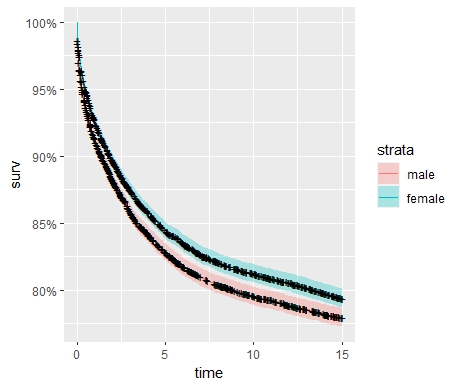
\includegraphics{sex}
\end{center}

When plotting the results, we can see that male children have a slightly lower rate of survival compared to female children.

\begin{center}
	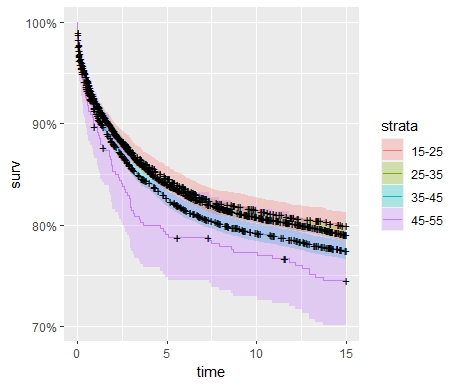
\includegraphics{m.age}
\end{center}

In order to plot the effect of the mother's age, i binned the column into the categories 15-25, 25-35, 35-45 and 45-55. This allows us to compare survival rates for the children of differently aged mothers.

	\lstinputlisting[language=R, firstline=72,lastline=76]{PS4_VD17341481.R} 

As the results in the table showed, the older the mother, the lower the rate of survival for children.

\end{document}
